\chapter{Results}
\label{ch:results}
\thispagestyle{fancy}

    Although ANOVA models are commonly used in behavioral sciences when analyzing treatment differences in repeated measures, several authors have question their adequacy (\cite{camilli1987}, \cite{vasey1987}, \cite{jaeger2008}, \cite{locker2007}, \cite{krueger2004}). Specially critical in my design is the fact that participants are matched in groups which do not change during the experiment but may develop their own dynamic. Imagine for instance a group in which the majority of participants are very risk friendly or have a high valuation. Investments might increase in total, even for those participants that are not as risk friendly.\\ 
    
    Instead, linear mixed models as used for instance in \cite{szaszi2018}, \cite{holsen2009} or \cite{yue2010} are encouraged since they allow to study the general effect of the variables of interest while allowing random intercepts for groups and participants while taking into account the auto-correlation of the repeated measure (\cite{galecki2013}, \cite{bolker2009}, \cite{mcculloch2015}, \cite{barr2013}, \cite{baayen2008}, \cite{fitzmaurice2015}). I therefore generally use a linear mixed model specification to be compared against a so-called "fixed effects" only model in the result analysis below. If not indicated otherwise, I chose the model using Akaike's Information Criterion.\\

    All the data preparation, analysis and visualization was done using the statistical software \textit{R}\footnote{and the packages \textit{tidyverse} \citep{wickham2017b}, \textit{data.table} \citep{dowle2018}, \textit{ineq} \citep{zeileis2014}, \textit{stargazer} \citep{hlavac2018}, \textit{ggplot2} \citep{wickham2016}, \textit{sjstats} \citep{ludecke2018}, \textit{texreg} \citep{leifeld2013}, \textit{ggthemes} \citep{arnold2018}, \textit{ggridges} \citep{wilke2018}, and others which are referenced in due course.} \citep{rcoreteam2014}. All data, scripts and results are available at XXX.XXX.XXX, even those that for space reasons were not included in the print version of this thesis.

\section{Benchmarking }

During the benchmarking rounds, participants solved around 10 sequences with the piece rate of one token per sequence. With the high piece rate of two tokens per sequence, participants solved an average of 15.3 sequences. The mean valuation, that is, the mean difference between the earnings (income from solving sequences plus income from the leisure mode) in the low and the high piece rate were of around 13 tokens. Table \ref{tab:avg_prod_bench} summarises this findings.\\

\begin{table}[!htbp] \centering 
  \caption{Mean Values of Production in Benchmark} 
  \label{tab:avg_prod_bench} 
\begin{tabular}{@{\extracolsep{5pt}} cccc} 
\\[-1.8ex]\hline 
\hline \\[-1.8ex] 
treatment & avg. prod. low wage & avg. prod. high wage & mean valuation \\ 
\hline \\[-1.8ex] 
0 & 9.77 & 15.29 & 12.9 \\ 
1 & 10.25 & 15.29 & 13.09 \\ 
\hline \\[-1.8ex] 
\end{tabular} 
\end{table} 

\section{Competition}
\subsection{Sequence Production \& Income}
\label{sec:seq_prod}
Participants solved an average of 11.5 sequences in the competition rounds and spent an average of 85.2 seconds in the \textit{switch} mode. There was little difference in production between wages, i.e. between winners and losers, but some difference can be observed between treatments. Subjects in the treatment produced less in average and spent more time in the \textit{switch} mode. Table \ref{tab:avg_prod} and graph \ref{fig:production_boxplot} summarize these findings.\\

\begin{table}[!htbp] \centering
  \caption{Mean Values of Production\\
    \footnotesize{standard errors are reported in parentheses ()}} 
  \label{tab:avg_prod}
\begin{tabular}{@{\extracolsep{5pt}} cccc} 
\\[-1.8ex]\hline 
\hline \\[-1.8ex] 
treatment & wage & mean solved sequences & mean of time spent in switch \\ 
\hline \\[-1.8ex] 
0 & 1 & 12.02 & 78.66 \\ 
 &  & (0.23) & (3.13) \\ 
0 & 2 & 11.91 & 79.09 \\
 &  & (0.3) & (4.22) \\ 
1 & 1 & 11.1 & 92.28 \\
 &  & (0.21) & (2.86) \\ 
1 & 2 & 11.12 & 90.23 \\
 &  & (0.33) & (4.42) \\ 
\hline \\[-1.8ex]
\end{tabular}
\end{table}  

\begin{figure}
    \centering
    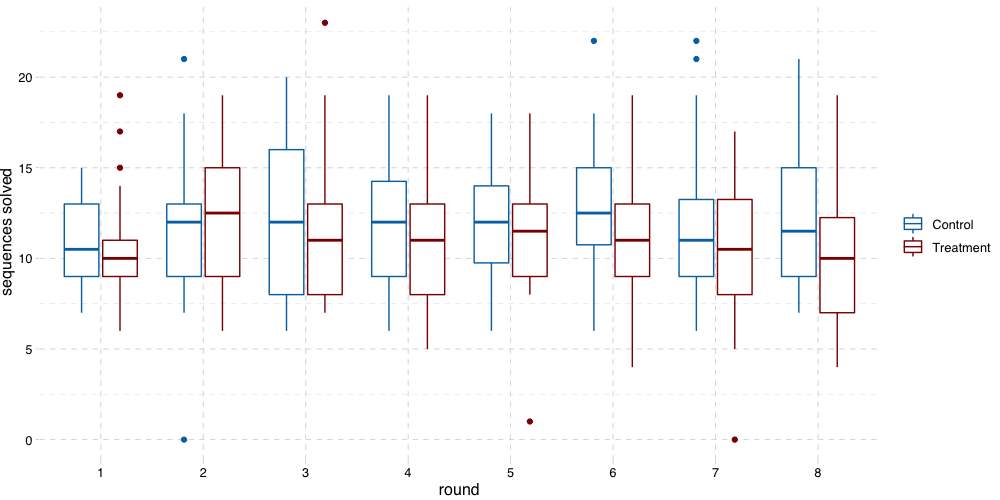
\includegraphics[width=\textwidth]{graphs/production_boxplot.png}
    \caption{Number of Sequences Solved per Round and Treatment}
    \label{fig:production_boxplot}
\end{figure}

To see if the difference in production between the treatments is statistically significant, and to see how other factors play a role, I used a linear mixed model (LMM) with random intercepts evaluated using the \textit{R} package \textit{lme4} \citep{bates2015}. Since the design allows only for between-groups comparisons regarding the treatment, I exclude a random slope per participant, assuming thus that the effect of time will be equivalent for all subjects.\\ 

In this model, the fixed effects are the \textit{treatment}, \textit{was winner} (if a participant won the previous round and is playing with the high wage), and the \textit{round} number. The random effect is the \textit{subjects id} nested within the \textit{group}. Results are reported following largely \cite{barr2013} and are summarized in table \ref{table:lmer_prod}. P-values were calculated using the likelihood ratio test of the \textit{R} package \textit{lmerTest} \citep{kuznetsova2017}.\\

\textit{Treatment} has a small although significant effect at the 0.1 level with subjects in the control group solving just shy of 1 sequence more per round. All the other fixed effects have no significant or large effect with the model in total explaining 42\% of the observed variance in which the fixed effects explain 1.52\% (conditional R-squared and marginal r-squared respectively, calculated using the \textit{psycho} package \citep{makowski2018}). This includes, interestingly, the wage at which participants played.\\

Note that although the residual plot and qq-plot do not make apparent any deviation from a normal distribution nor any systematic increase or decrease in variance, there is much debate as to how to appropriately check for the validity of assumptions in LMMs  \citep{loy2017}, specially when dealing with distributions other than normal, and will therefore be left out for now in this thesis.\\

\begin{table}[!htbp] \centering 
  \caption{Linear Mixed Model - Sequence Production} 
  \label{table:lmer_prod} 
  \scalebox{0.8}{%
\begin{tabular}{@{\extracolsep{5pt}}lc} 
\\[-1.8ex]\hline 
\hline \\[-1.8ex] 
 & \multicolumn{1}{c}{\textit{Dependent variable:}} \\ 
\cline{2-2} 
\\[-1.8ex] & Sequence Production \\ 
\hline \\[-1.8ex] 
 treatment & $-$0.872$^{*}$ \\ 
  & (0.499) \\ 
  & \\ 
 was winner & 0.028 \\ 
  & (0.231) \\ 
  & \\ 
 round & $-$0.003 \\ 
  & (0.043) \\ 
  & \\ 
 Constant & 11.985$^{***}$ \\ 
  & (0.408) \\ 
  & \\ 
\hline \\[-1.8ex] 
Observations & 768 \\ 
Log Likelihood & $-$1,943.528 \\ 
Akaike Inf. Crit. & 3,901.055 \\ 
Bayesian Inf. Crit. & 3,933.525 \\
\hline \\ [-1.8ex] 
Var: participant|group (Intercept) & 5.08\\
Var: group (Intercept) & 0.00 \\
Var: Residual & 7.28 \\
\hline \\[-1.8ex] 
\hline 
\textit{Note:}  & \multicolumn{1}{r}{$^{*}$p$<$0.1; $^{**}$p$<$0.05; $^{***}$p$<$0.01} \\ 
\end{tabular}
}
\end{table} 

Remember that in this experimental design, payoffs are not exclusively determined by the amount of sequences solved. They depend also on time spent in the \textit{switch} mode and therefore on the optimal change to it; the invested amount in human capital, and, in the treatment, how much the other players worked. The boxplot in figure \ref{fig:earnings_boxplot} seems to suggest that net income is higher in the treatment groups and that, apart from round 1, they do not change over time. Note that net income describes here income after taxation AND redistribution but before investment. To see if there were significant differences, I use a model with fixed effects \textit{treatment, was winner} and \textit{round} and summarise the findings in table \ref{table:earnings_lmer}.\\

Winning the previous round, i.e. playing with the high wage has a strong and significant effect on net income while time, although slightly significant, has only a small effect. The introduction of a tax and redistribution scheme, on the other hand, does not have a significant effect. The model helps explaining 50.11\% (restricted r-squared) of the variance with the fixed effects accounting for 33.73\% (marginal r-squared) of the variance.\\

Notice that while the taxation treatment has a negative impact on the number of sequences solved, it has a non-significant positive effect on net income. This is an indication that participants were over-performing in the control and, when confronted with a redistribution scheme, diminished their production such that the moment of switching to the leisure mode was closer to the optimum. Thus, earning relatively equal despite the effective tax rate of 40\%.\\

\begin{figure}
    \centering
    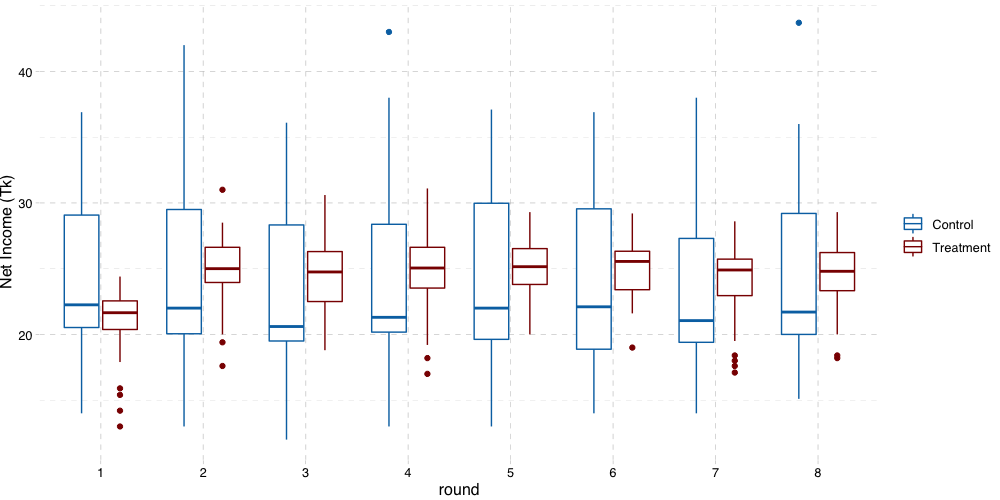
\includegraphics[width=\textwidth]{graphs/earnings_boxplot.png}
    \caption{Income after Taxation and Redistribution, and before investment}
    \label{fig:earnings_boxplot}
\end{figure}


\begin{table}[!htbp] \centering 
  \caption{Linear Mixed Model - Net Income} 
  \label{table:earnings_lmer}
  \scalebox{0.8}{%
\begin{tabular}{@{\extracolsep{5pt}}lc} 
\\[-1.8ex]\hline 
\hline \\[-1.8ex] 
 & \multicolumn{1}{c}{\textit{Dependent variable:}} \\ 
\cline{2-2} 
\\[-1.8ex] & net income \\ 
\hline \\[-1.8ex] 
 treatment & 0.598 \\ 
  & (0.471) \\ 
  & \\ 
 was winner & 5.977$^{***}$ \\ 
  & (0.289) \\ 
  & \\ 
 round & 0.090$^{*}$ \\ 
  & (0.054) \\ 
  & \\ 
 Constant & 21.434$^{***}$ \\ 
  & (0.422) \\ 
  & \\ 
\hline \\[-1.8ex] 
Observations & 768 \\ 
Log Likelihood & $-$2,098.867 \\ 
Akaike Inf. Crit. & 4,211.735 \\ 
Bayesian Inf. Crit. & 4,244.241 \\ 
\hline 
Var: participant|group (Intercept) & 3.86          \\
Var: group (Intercept)           & 0.00          \\
Var: Residual                              & 11.77         \\
\hline
\hline \\[-1.8ex] 
\textit{Note:}  & \multicolumn{1}{r}{$^{*}$p$<$0.1; $^{**}$p$<$0.05; $^{***}$p$<$0.01} \\ 
\end{tabular}
}
\end{table} 


\subsection{Optimum of Work Supply}
During the competition, participants tend to work more than their optimum. Remember, participants should switch as soon as the time they need to solve a given task surpasses the earnings in the switch mode for the corresponding time. In the control group, players with the low wage should change as soon as they take longer than 10 seconds to solve the task, in the treatment, as soon as they need more than six seconds. In each treatment, players with the high wage should switch at twice the respective time. Graph \ref{fig:time_per_task} shows the time needed for each task per round and marks the 10 and 20 seconds cutoffs.\\

It seems in fact as if the time needed to solve each sequence is more compressed to the middle in the treatment. Table \ref{table:earnings_lmer} offers a strong indication in this direction as explained at the end of section \ref{sec:seq_prod}. However, a Wilcoxon test cannot reject the null hypothesis (p: 0.283) of no shift regarding the overall seconds over the 10 or 20 cutoffs. In chapter \ref{ch:conclusion} I address a design change that could make it easier to identify if there are general changes to the switching point when taxation is introduced.\\

\begin{figure}
    \centering
    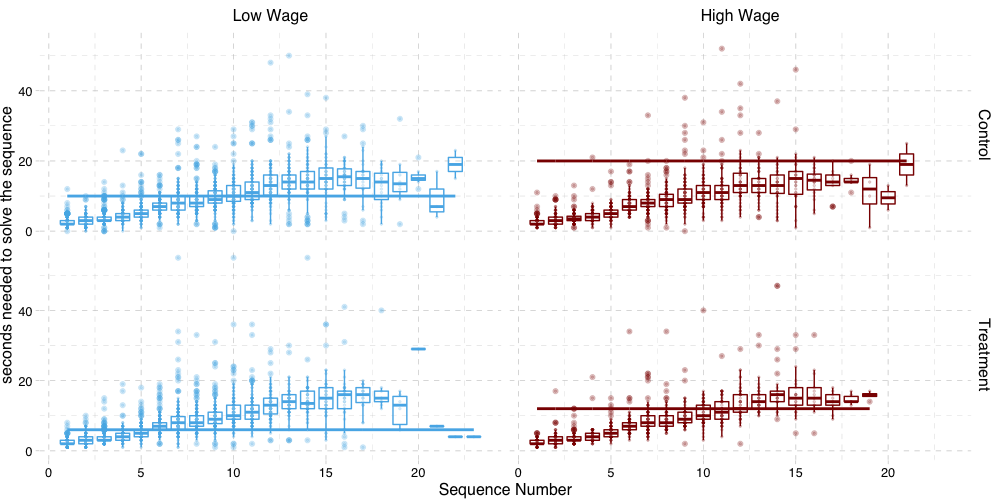
\includegraphics[width=\textwidth]{graphs/time_task_grid.png}
    \caption{Count of Choice of Switching Row}
    \label{fig:time_per_task}
\end{figure}

\section{Controls}

\subsection{Cognitive Reflection Test}
In the \textit{Cognitive Reflection Test}, participants answered, out of 4, in average 2.22 (s.e. 0.1) questions correctly. Men answered in average 0.3 (s.e. 0.15) more questions correctly with women giving 2.09 (s.e. 0.13) right answers in average.\\


\subsection{Risk Elicitation Task}
In the \textit{Risk Elicitation} task, participants chose in average row 6.6 to switch, which according to table \ref{table:HL} indicates a risk averse to very risk averse behaviour. Men generally showed a more risk averse behaviour, switching in average at row 6.93 (s.e. 0.32), while women switched in average already at row 6.36 (s.e. 0.33). Figure \ref{fig:hist_mpl} shows a histogram of the row at which participants switched.\\

\begin{figure}
    \centering
    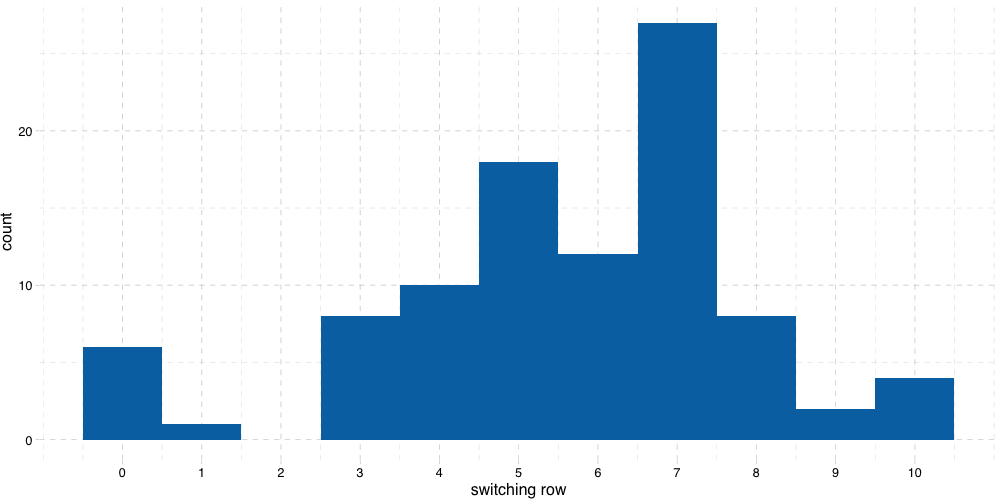
\includegraphics[width=\textwidth]{graphs/hist_mpl.png}
    \caption{Count of Choice of Switching Row}
    \label{fig:hist_mpl}
\end{figure}

\subsection{Fairness Sentiment}

Participants did not seem to change their views on the fairness of the game. Figure \ref{fig:fairness_boxplot} shows a boxplot of their assessment at the beginning and at the end of the competition rounds. Table \ref{tab:fair_ols} shows a linear regression that shows no apparent significant influence in changing a participant's view on fairness.\\

\begin{figure}
    \centering
    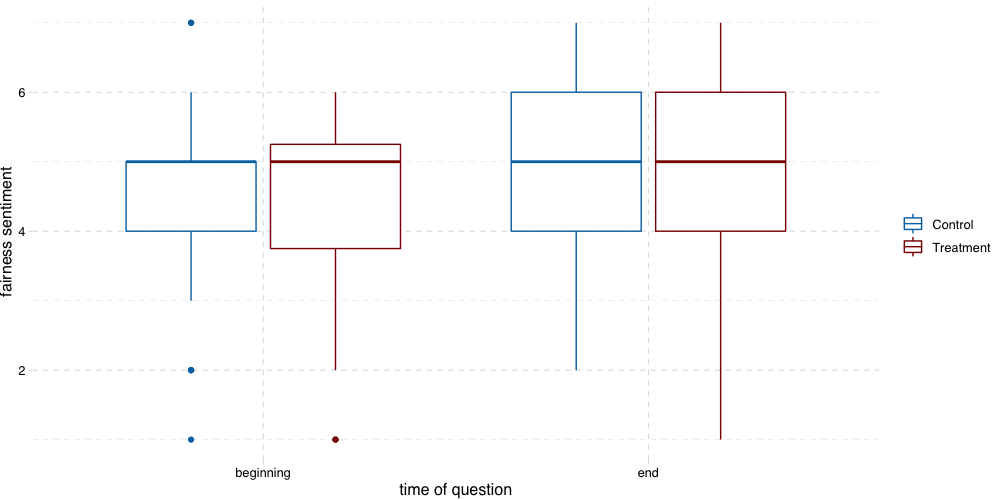
\includegraphics[width=\textwidth]{graphs/fairness_sentiment_boxplot.png}
    \caption{Fairness Sentiment Voting}
    \label{fig:fairness_boxplot}
\end{figure}



\begin{table}[!htbp] \centering 
  \caption{OLS Change in Fairness Sentiment} 
  \label{tab:fair_ols} 
\begin{tabular}{@{\extracolsep{5pt}}lc} 
\\[-1.8ex]\hline 
\hline \\[-1.8ex] 
\\[-1.8ex] & Change in Fairness Sentiment \\ 
\hline \\[-1.8ex] 
 treatment & $-$0.183 \\ 
  & (0.391) \\ 
  & \\ 
 payoff & 0.015 \\ 
  & (0.052) \\ 
  & \\ 
 crt score & 0.063 \\ 
  & (0.188) \\ 
  & \\ 
 switching row & 0.013 \\ 
  & (0.084) \\ 
  & \\ 
 gender (Male) & $-$0.181 \\ 
  & (0.366) \\ 
  & \\ 
 valuation & 0.048 \\ 
  & (0.063) \\ 
  & \\ 
 Constant & $-$0.971 \\ 
  & (1.298) \\ 
  & \\ 
  \hline
Observations & 96 \\ 
R$^{2}$ & 0.016 \\ 
Adjusted R$^{2}$ & $-$0.051 \\ 
Residual Std. Error & 1.733 (df = 89) \\ 
F Statistic & 0.235 (df = 6; 89) \\ 
\hline \\[-1.8ex] 
\textit{Notes:} & \multicolumn{1}{l}{$^{***}$Significant at the 1 percent level.} \\ 
 & \multicolumn{1}{l}{$^{**}$Significant at the 5 percent level.} \\ 
 & \multicolumn{1}{l}{$^{*}$Significant at the 10 percent level.} \\ 
\end{tabular} 
\end{table} 

\section{Hypotheses Testing}

In this section we will have a look at the results regarding, one, the distribution of probabilities and its change across rounds, and, second, the factors affecting the probability of winning for a given individual according to the hypotheses postulated in section \ref{ss:hyp}.


\subsection{Hypotheses 1 and 2}

\textbf{Hypothesis \ref{hyp:treat}} \textit{Mean investments will be higher than the expected profit maximizing value for all treatments, but decreasing over time.}\\ 
\textbf{Hypothesis \ref{hyp:treat-overinvest}} \textit{Participants in the treatment will invest a lower share of their optimal investment}\\

To test this hypotheses, I firstly need to determine the optimal investment value for each participant. Assuming an equal valuation for all participants in a given treatment greatly simplifies the process by allowing to use formula \ref{eq:opt_last}. Running a t-test on the hypothesis that the distance to the mean is 0, supports this assumption (p: 1 for control and p: 0.85 for the treatment).\\

Furthermore, since the treatment and control groups have different valuations, to easier interpret the results I analyze the mean difference over optimal investment for both groups instead of the nominal amount of over-investment. Note that in comparison to table \ref{tab:avg_prod_bench}, the valuation for the treated groups is calculated from the difference in the taxed benchmark rounds as explained in section \ref{ss:tax_bench}.\\

Participants appear to invest less with each round as the histogram in graph \ref{fig:invest_hist} shows. Several participants indeed do not invest anything at all and this number increases with each repetition. Leading to the patter shown in figure \ref{fig:invest_prob_point}. With increasing rounds, the relationship between the invested amounts and the probability obtained grew apart. On the one hand with each round there were more high investments, while, on the other hand, more low investments achieved a high probability of winning.\\

\begin{figure}
    \centering
    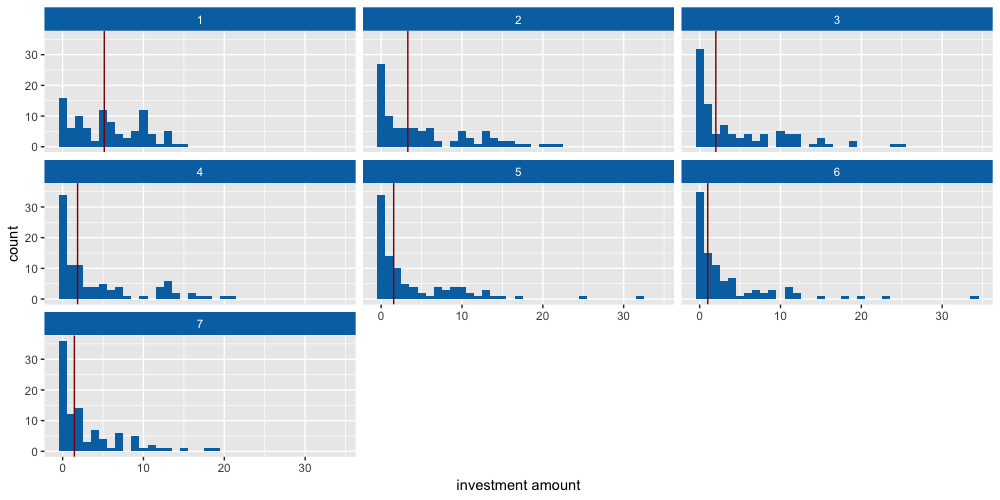
\includegraphics[width=\textwidth]{graphs/investment_amount_hist.png}
    \caption{Histogram of investment amounts faceted by round. The red line demarks the median of the distribution.}
    \label{fig:invest_hist}
\end{figure}

\begin{figure}
    \centering
    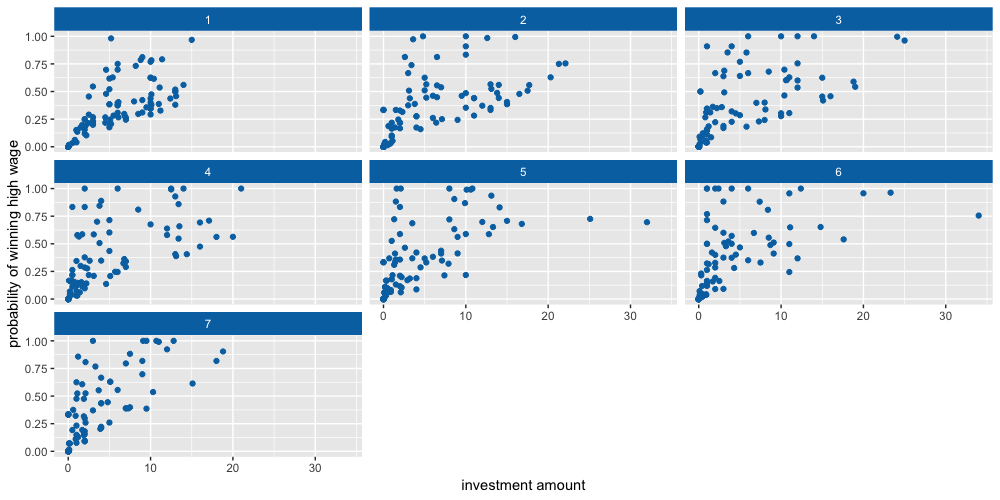
\includegraphics[width=\textwidth]{graphs/invest_prob_point.png}
    \caption{Plot of the probability achieved by a given investment faceted by round}
    \label{fig:invest_prob_point}
\end{figure}

Consistent with expectations, participants bid in average significantly more than their optimum but decreasingly so over time. Interestingly, participants in the taxation treatment invest both nominally and relatively more than those in the control, with treatment participants bidding in average 5 and a half times their optimal investment in the first round and 2.3 times their optimum in the last round. Participants in the control, on the other hand, invest from 1.93 times their optimum in the first round, to 1.36 times in the last round.\\


\begin{figure}
    \centering
    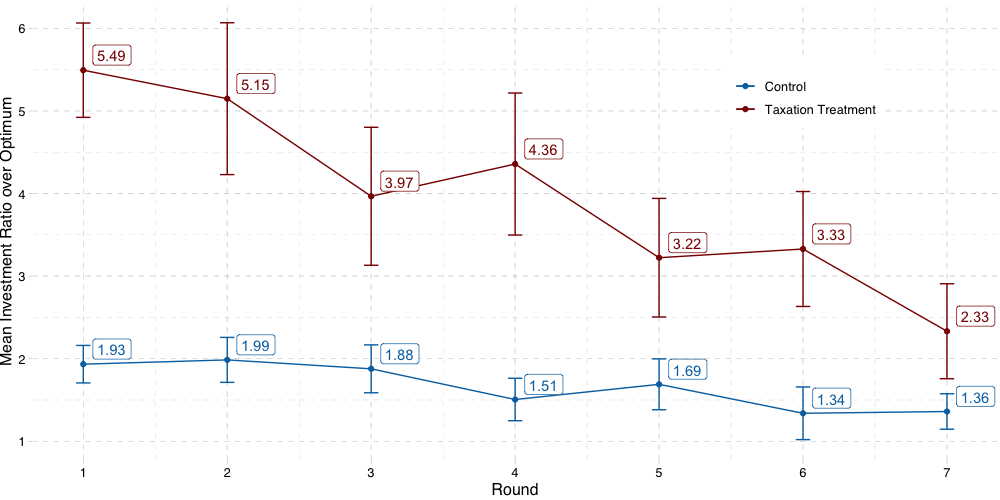
\includegraphics[width=\textwidth]{graphs/over_invest.png}
    \caption{Ratio of Over Investment per Round}
    \label{fig:over_invest}
\end{figure}

Table \ref{tab:over_invest} present a linear mixed model dissecting the most important effects on over-investing. The random effects are \textit{participants} nested in the \textit{group}.\\

\begin{table} \centering 
  \caption{Linear Mixed Model Over Investment Ratio} 
  \label{tab:over_invest}
  \scalebox{0.7}{%
\begin{tabular}{@{\extracolsep{5pt}}lcc} 
\\[-1.8ex]\hline 
\hline \\[-1.8ex] 
\\[-1.8ex] & \multicolumn{2}{c}{Ratio of Investment Over Optimum} \\ 
\\[-1.8ex] & (1) & (2)\\ 
\hline \\[-1.8ex] 
 treatment & 2.314$^{***}$ & 2.075$^{***}$ \\ 
  & (0.698) & (0.678) \\ 
  & & \\ 
 round & $-$0.307$^{***}$ & $-$0.307$^{***}$ \\ 
  & (0.055) & (0.055) \\ 
  & & \\ 
 was winner & 0.256 & 0.281 \\ 
  & (0.271) & (0.271) \\ 
  & & \\ 
 CRT score &  & $-$0.183 \\ 
  &  & (0.289) \\ 
  & & \\ 
 switching row &  & $-$0.375$^{***}$ \\ 
  &  & (0.126) \\ 
  & & \\ 
 gender (Male) &  & 0.284 \\ 
  &  & (0.583) \\ 
  & & \\ 
 Constant & 2.813$^{***}$ & 5.689$^{***}$ \\ 
  & (0.546) & (1.097) \\ 
  & & \\ 
  \hline
  \hline
Observations & 672 & 672 \\ 
Log Likelihood & $-$1,751.726 & $-$1,747.753 \\ 
Akaike Inf. Crit. & 3,517.453 & 3,515.506 \\ 
Bayesian Inf. Crit. & 3,549.024 & 3,560.608 \\
\hline
Var: participant|group (Intercept) & 5.66 &     5.17     \\
Var: group (Intercept)           & 1.62  &    1.48    \\
Var: Residual                              & 8.14   &   8.14    \\
\hline \\[-1.8ex] 
\textit{Notes:} & \multicolumn{2}{l}{$^{***}$Significant at the 1 percent level.} \\ 
 & \multicolumn{2}{l}{$^{**}$Significant at the 5 percent level.} \\ 
 & \multicolumn{2}{l}{$^{*}$Significant at the 10 percent level.} \\ 
\end{tabular}
}
\end{table}

The first and second models have a total explanatory power of around 52\% (conditional r-squared) in which the fixed effects of the first explain 10.03\% and the second 14.5\% of the variance (marginal r-squared). The effect of the treatment is significant and large for both models with participants investing, contrary to hypothesis \ref{hyp:treat-overinvest}, almost double as much as the control. Round repetition and risk averse behavior have both a significant although relatively small effect in the expected negative direction. The CRT score and whether a participant was playing with a high wage did not have a significant effect on the over-investment ratio.\\

Figure \ref{fig:beliefs_smooth} shows a reduction in the mean over-estimation of investments by the other group participants indicating better knowledge of other's behaviour with progressing rounds. It is nevertheless surprising how little accuracy participants appear to reach after playing seven rounds and having been shown all relevant information.\\

\begin{figure}
    \centering
    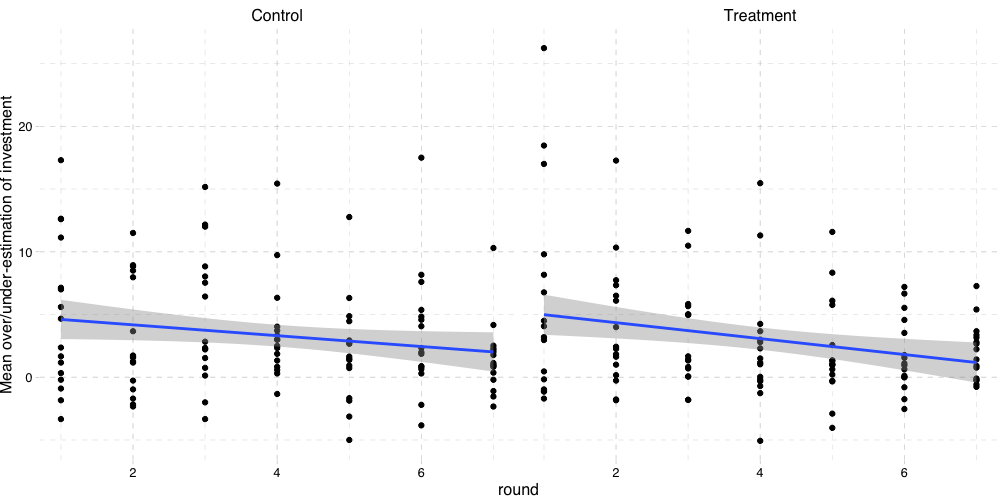
\includegraphics[width=\textwidth]{graphs/beliefs_smooth_lm.png}
    \caption{Mean Over or Under-estimation of other's investments by group and round}
    \label{fig:beliefs_smooth}
\end{figure}

A possibility for why participants in the treatment invest relatively more is that participants apply a heuristic of a fix proportion of available income for investment. Running a similar regression as above on the investment ratio of available income in fact deletes the effect of all fixed effects but time, suggesting that participants tend to invest the same amount of their available income, regardless of their earnings or idiosyncratic features. Figure \ref{fig:invest_share} shows a plot of the mean shares of the available income invested. The shares decrease with time in similar fashion for both treatments and apart from the final investing round, within an standard error from each other.\\

\begin{figure}
    \centering
    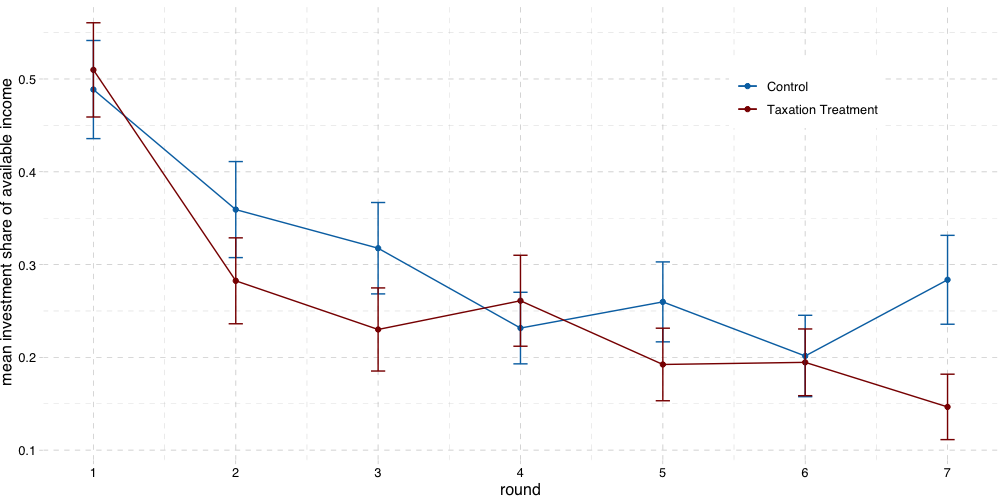
\includegraphics[width=\textwidth]{graphs/investment_share_geom_line.png}
    \caption{Investment share of available income per round}
    \label{fig:invest_share}
\end{figure}

A Wilcoxon rank test (p: 0.01) suggests furthermore that total welfare (the total amount of tokens payed out during competition) is larger in the treatment than in the control. Higher welfare in the treatment seems to be driven by working closer to the optimum. Adding the gini coefficient of the available income to the model in table \ref{tab:over_invest} does not show any significance of inequality nor does it change the remaining coefficients which strengthens the idea that the higher investment in the treatment is due to an available income share heuristic.\\



\subsection{Hypothesis 3}

\textbf{Hypothesis \ref{hyp:wins}} \textit{The coefficient of variance of winning probabilities will be increasing across rounds while being smaller in the treatment.}\\

In terms of probabilities, I am interested in how its distribution change. Naturally, the mean probability of earning the high wage is always equal to $1/n$, but its distribution can vary from exactly $1/n$ for each participant, to only one person in the group having a probability of 1 and all the rest a probability of 0. Figure \ref{fig:dens_prob} shows the density plots for each round. A completely equal distribution would have its maximum at 0.33 with no values around it, while a completely unequal distribution would see two peaks at each extreme with the one at 0 being twice the size of the the one at 1.\\

\begin{figure}[H]
    \centering
    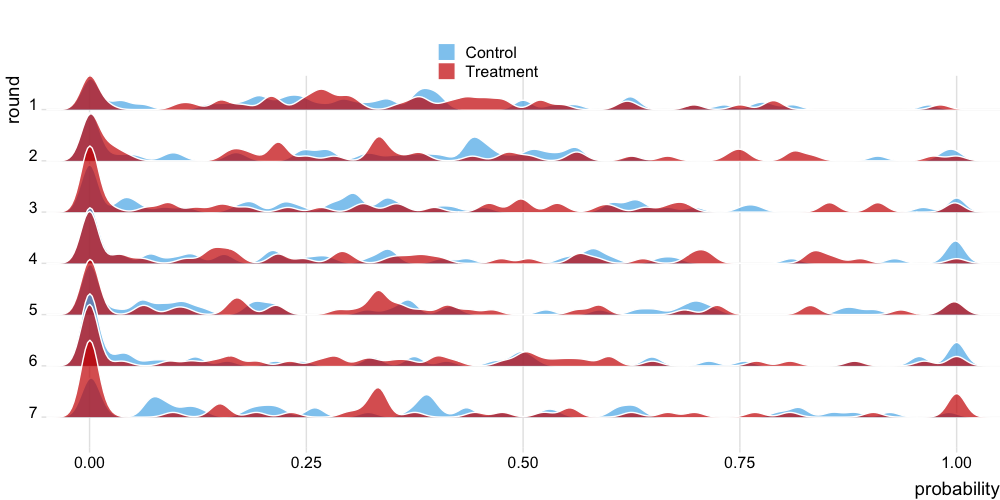
\includegraphics[width = \textwidth]{graphs/density_ridge_prob.png}
    \caption{Density Plots of Probability across Rounds}
    \label{fig:dens_prob}
\end{figure}

Figure \ref{fig:dens_prob} seems in fact to show an increase of density at the ends of the distribution with round 1 having a rather flat shape and round 8 stronger peaks at both 0 and 1 probability. To test if the distribution of probabilities between the treatments really differ, I use the coefficient of variation $c_v=\frac{\sigma}{\mu}$ as for instance in \cite{rassenti2000}, as \cite{bendel1989} recommends it to use in cases where there is a relatively exact measure of the values. Figure \ref{fig:var_coeff_boxplot} shows a box plot of the coefficient of variations across rounds for both treatments. In fact, it seems to increase across rounds but not significantly so between treatments.\\

\begin{figure}[H]
    \centering
    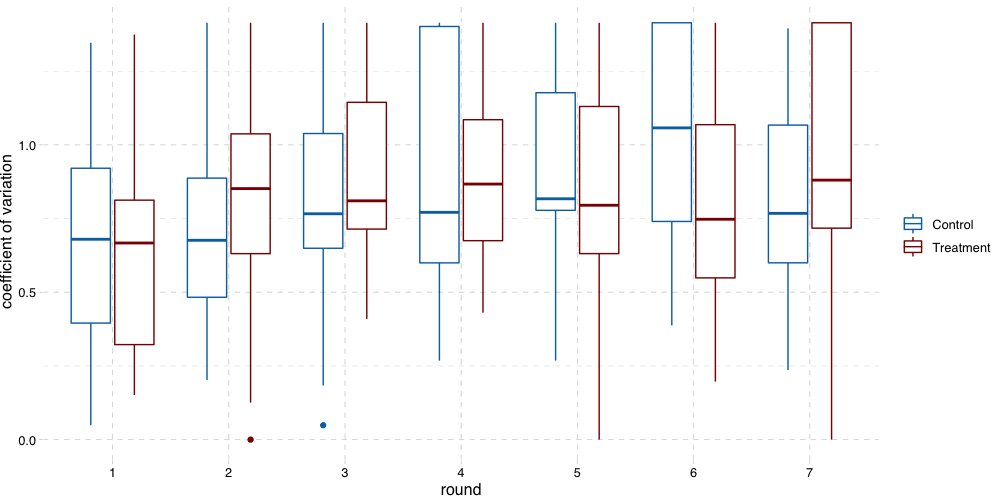
\includegraphics[width = \textwidth]{graphs/var_coeff_prob_boxplot.png}
    \caption{Boxplot Coefficient of Variation}
    \label{fig:var_coeff_boxplot}
\end{figure}

Table \ref{tab:var_coeff_ols} shows the results for an OLS regression of two models explaining the difference across groups in the coefficient of variation for the probabilities of winning. A linear mixed model is left out here since each group is part of only one treatment and the variables are all aggregated at the group level. Only round repetition appears to have a significant, although small effect (in our setting, the coefficient of variance can fluctuate between 0 and 1.73) on the coefficient of variation. Idiosyncratic group values like the mean value of valuation, CRT score or risk aversion do not play a significant role in the variation of probabilities. Taxation and redistribution also do not play a role. In other words, introducing a redistribution scheme does not avoid the fact that, with time, the distribution of probabilities will go to extremes with some participants having most of the chance to win and the rest having almost none.\\


\begin{table}[!htbp] \centering 
  \caption{OLS Coefficient of Variation} 
  \label{tab:var_coeff_ols} 
\begin{tabular}{@{\extracolsep{5pt}}lcc} 
\\[-1.8ex]\hline 
\hline \\[-1.8ex] 
\\[-1.8ex] & \multicolumn{2}{c}{Probability Coefficient of Variation} \\ 
\\[-1.8ex] & (1) & (2)\\ 
\hline \\[-1.8ex] 
 treatment & $-$0.025 & $-$0.031 \\ 
  & (0.063) & (0.065) \\ 
  & & \\ 
 round & 0.043$^{***}$ & 0.043$^{***}$ \\ 
  & (0.016) & (0.016) \\ 
  & & \\ 
 mean CRT score &  & 0.092 \\ 
  &  & (0.059) \\ 
  & & \\ 
 mean switching row &  & $-$0.020 \\ 
  &  & (0.025) \\ 
  & & \\ 
 mean valuation &  & $-$0.033 \\ 
  &  & (0.023) \\ 
  & & \\ 
 Constant & 0.856$^{***}$ & 1.218$^{***}$ \\ 
  & (0.077) & (0.338) \\ 
  & & \\
  \hline
Observations & 224 & 224 \\ 
R$^{2}$ & 0.034 & 0.053 \\ 
Adjusted R$^{2}$ & 0.025 & 0.031 \\ 
Residual Std. Error & 0.468 (df = 221) & 0.467 (df = 218) \\ 
F Statistic & 3.857$^{**}$ (df = 2; 221) & 2.431$^{**}$ (df = 5; 218) \\ 
\hline \\[-1.8ex] 
\textit{Notes:} & \multicolumn{2}{l}{$^{***}$Significant at the 1 percent level.} \\ 
 & \multicolumn{2}{l}{$^{**}$Significant at the 5 percent level.} \\ 
 & \multicolumn{2}{l}{$^{*}$Significant at the 10 percent level.} \\ 
\end{tabular} 
\end{table}

Of course, this does not tell us much about what determines the probability of a given participant to win a contest. To analyze it, I suggest again a linear mixed model although this time a generalized mixed model from a beta distribution\footnote{Since several participants did not invest at all and thus had a probability of winning of 0, leading to some other participants to have a probability of winning of 1, those values were transformed to 0.0000000000001 and 0.0000000000009 respectively to allow to fit a beta distribution.}. Table \ref{tab:glm_prob} shows the results.\\

The only variable that shows a significant, although small, effect on the probability of winning is the size of the available income. Note in particular, that having won alone has no significant effect on the probability of winning. This is in part because participants can still have a large available income if they forfeit time in the leisure mode. An alternative model including cumulative wins also showed no influence on the probability of winning.\\

\begin{table}[!htbp] \centering 
  \caption{GLMM Probability of Winning} 
  \label{tab:glm_prob} 
\begin{tabular}{@{\extracolsep{5pt}}lcc} 
\\[-1.8ex]\hline 
\hline \\[-1.8ex] 
\\[-1.8ex] & \multicolumn{2}{c}{Probability of Winning} \\ 
\\[-1.8ex] & (1) & (2)\\ 
\hline \\[-1.8ex] 
 treatment & $-$0.139 &  $-$0.087241 \\ 
  & (0.22) & (0.218) \\ 
  & & \\ 
 available income & 0.045$^{***}$ & 0.045$^{***}$ \\ 
  & (0.008) & (0.008) \\ 
  & & \\ 
 was winner & $-$0.084 &  $-$0.083 \\ 
  & (0.119) & (0.119) \\ 
  & & \\ 
 gender (male) &  & 0.356 \\ 
  &  & (0.223) \\ 
  & & \\ 
 CRT Score &  & $-$0.051 \\ 
  &  & (0.113) \\ 
  & & \\ 
 switching row & & $-$0.034 \\ 
  &  & (0.049) \\ 
  & & \\ 
 valuation &  & 0.056 \\ 
  &  & (0.038) \\ 
  & & \\ 
 mean investment belief &  & 0.003 \\ 
  &  & (0.008) \\ 
  & & \\ 
 Constant & $-$1.413$^{***}$ & $-$2.454$^{***}$ \\ 
  & (0.209) & (0.647) \\ 
  & & \\ 
  \hline
Observations & 672 & 672 \\ 
Log Likelihood & 3798.4 & 3801.0 \\ 
Akaike Inf. Crit. & $-$7580.9 & $-$7575.9 \\ 
Bayesian Inf. Crit. & $-$7544.8 & $-$7517.3 \\
\hline
Num. groups: participant:group     & 96     &   96   \\
Num. groups: group               & 32      &    32  \\
Num. groups: round                         & 7   & 7        \\
\hline
Var: participant:group (Intercept) & 0.93   & 0.02     \\
Var: group (Intercept)           & 0.00   & 0.00     \\
Var: round (Intercept)           & 0.00    & 0.00    \\
Var: Residual                    & 0.00     &  0.02  \\
\hline
\hline \\[-1.8ex] 
\textit{Notes:} & \multicolumn{2}{l}{$^{***}$Significant at the 1 percent level.} \\ 
 & \multicolumn{2}{l}{$^{**}$Significant at the 5 percent level.} \\ 
 & \multicolumn{2}{l}{$^{*}$Significant at the 10 percent level.} \\ 
\end{tabular} 
\end{table} 